\documentclass[a4paper, 11pt]{article}
\usepackage{comment} 
\usepackage{fullpage}
\usepackage{amsmath} 
\usepackage{amssymb} 
\usepackage{mathtools}
\usepackage{siunitx}
\usepackage{xfrac}
\usepackage{icomma}
\usepackage[section,below]{placeins}
\usepackage[labelfont=bf,font=small,width=0.9\textwidth]{caption}
\usepackage{subcaption}
\usepackage{graphicx}
\usepackage{grffile}
\usepackage{float}
\floatplacement{figure}{htbp}
\floatplacement{table}{htbp}
\usepackage{booktabs}
\usepackage{hyperref}
\usepackage{pdfpages}
\sisetup{separate-uncertainty=true}

\begin{document}
\noindent
\centerline{\small{\textsc{Michigan State University}}} \\
\large{\textbf{CMSE 823 – Numerical Linear Algebra \hfill Spring 2020 \\
Homework 8}} \\
Alexander Harnisch \\
\noindent\makebox[\linewidth]{\rule{\textwidth}{0.4pt}}

\section*{1-4}
You can find my solutions in handwritten form included over the next few
pages. The code for the numerical part of Problem 1 is contained in
\textit{1.py}.
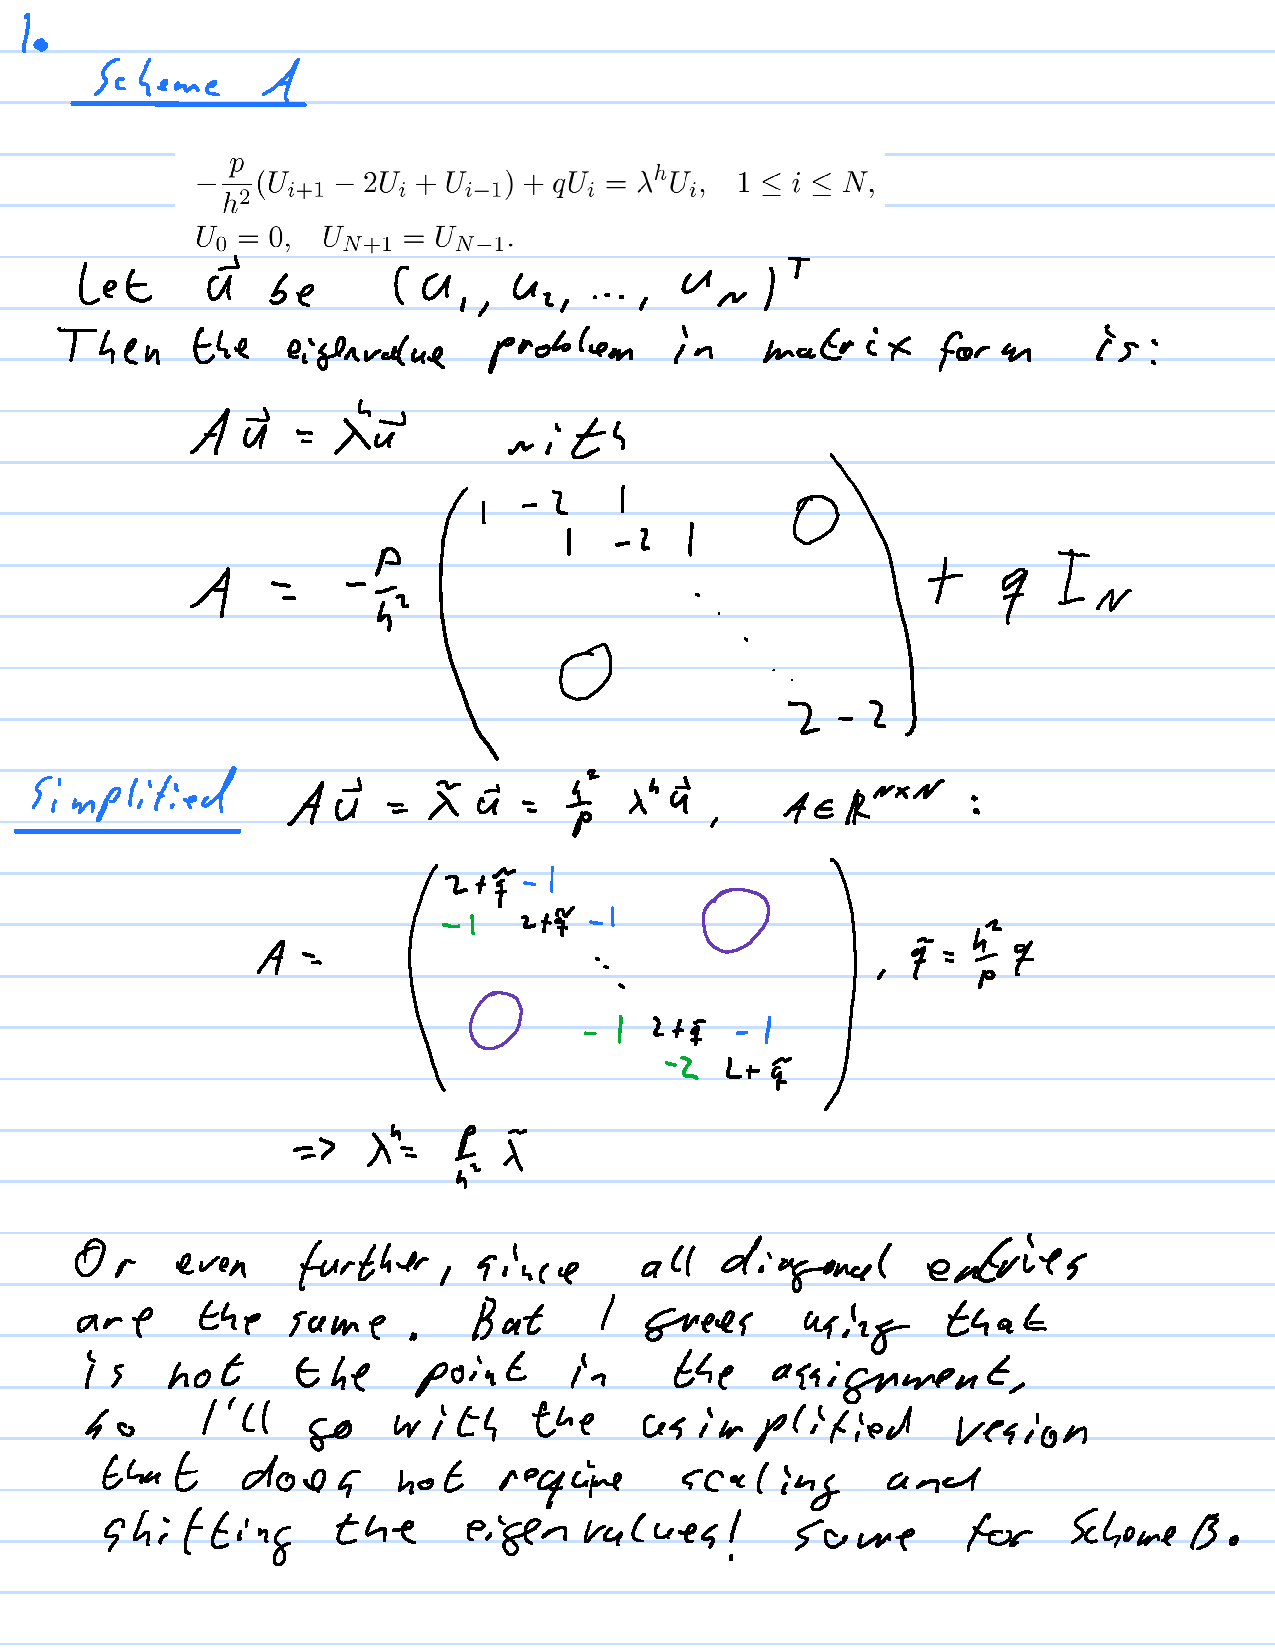
\includepdf[pages={1-8}]{../handwritten_part.pdf}

\FloatBarrier
\section*{5-7}
You can find the code in \textit{main.py} and \textit{solve.py}. The output for 5 and 6 is:
\begin{verbatim}
n = 2
-----
Gaussian Elimination:
x = [1. 1.]
L2-norm(x_true - x) = 8.005932084973442e-16
Cholesky Decomposition:
x = [1. 1.]
L2-norm(x_true - x) = 4.002966042486721e-16
QR Decomposition:
x = [1. 1.]
L2-norm(x_true - x) = 1.5895974606912448e-15

n = 4
-----
Gaussian Elimination:
x = [1. 1. 1. 1.]
L2-norm(x_true - x) = 7.55503627649389e-13
Cholesky Decomposition:
x = [1. 1. 1. 1.]
L2-norm(x_true - x) = 1.067152660435905e-12
QR Decomposition:
x = [1. 1. 1. 1.]
L2-norm(x_true - x) = 1.4414707055961225e-12

n = 6
-----
Gaussian Elimination:
x = [1. 1. 1. 1. 1. 1.]
L2-norm(x_true - x) = 6.164843591153147e-10
Cholesky Decomposition:
x = [1. 1. 1. 1. 1. 1.]
L2-norm(x_true - x) = 4.716983506492431e-10
QR Decomposition:
x = [1. 1. 1. 1. 1. 1.]
L2-norm(x_true - x) = 5.048570528880727e-11

n = 8
-----
Gaussian Elimination:
x = [1.         1.         0.99999998 1.00000013 0.99999966 1.00000049
 0.99999965 1.0000001 ]
L2-norm(x_true - x) = 7.087262141318325e-07
Cholesky Decomposition:
x = [1.         1.         0.99999994 1.00000031 0.99999915 1.0000012
 0.99999915 1.00000024]
L2-norm(x_true - x) = 1.740702948561934e-06
QR Decomposition:
x = [1.         1.         0.99999995 1.00000026 0.9999993  1.000001
 0.99999929 1.0000002 ]
L2-norm(x_true - x) = 1.4556315190530475e-06

n = 10
------
Gaussian Elimination:
x = [1.         1.00000011 0.99999774 1.00002048 0.99990264 1.00026691
 0.99956309 1.0004214  0.99977914 1.0000485 ]
L2-norm(x_true - x) = 0.00070763269657929
Cholesky Decomposition:
x = [1.         1.00000015 0.99999696 1.00002717 0.99987216 1.00034741
 0.99943562 1.00054075 0.99971824 1.00006155]
L2-norm(x_true - x) = 0.0009120887496429259
QR Decomposition:
x = [1.         1.00000004 0.9999992  1.00000687 0.99996892 1.0000816
 0.99987143 1.00011988 0.99993904 1.00001303]
L2-norm(x_true - x) = 0.00020605530255466347
\end{verbatim}
A visualization of the results is given in Figre~\ref{fig:7}. The error
expressed as the norm $\Vert x_\textup{True} - x \Vert_2$ grows exponentially
(as expected) with the order $n$ of the Hilbert matrix. I can not see any
significant trend in the difference between the 3 methods though. The
assignment asks for `` pertinent comments on these methods'', I don't know what
else there is to say. There does not seem to be any difference in accuracy.
Obviously the runtime is different for all methods with Gaussian Elimination
being the most efficient one, as discussed in detail in the textbook.
\begin{figure}
  \centering
  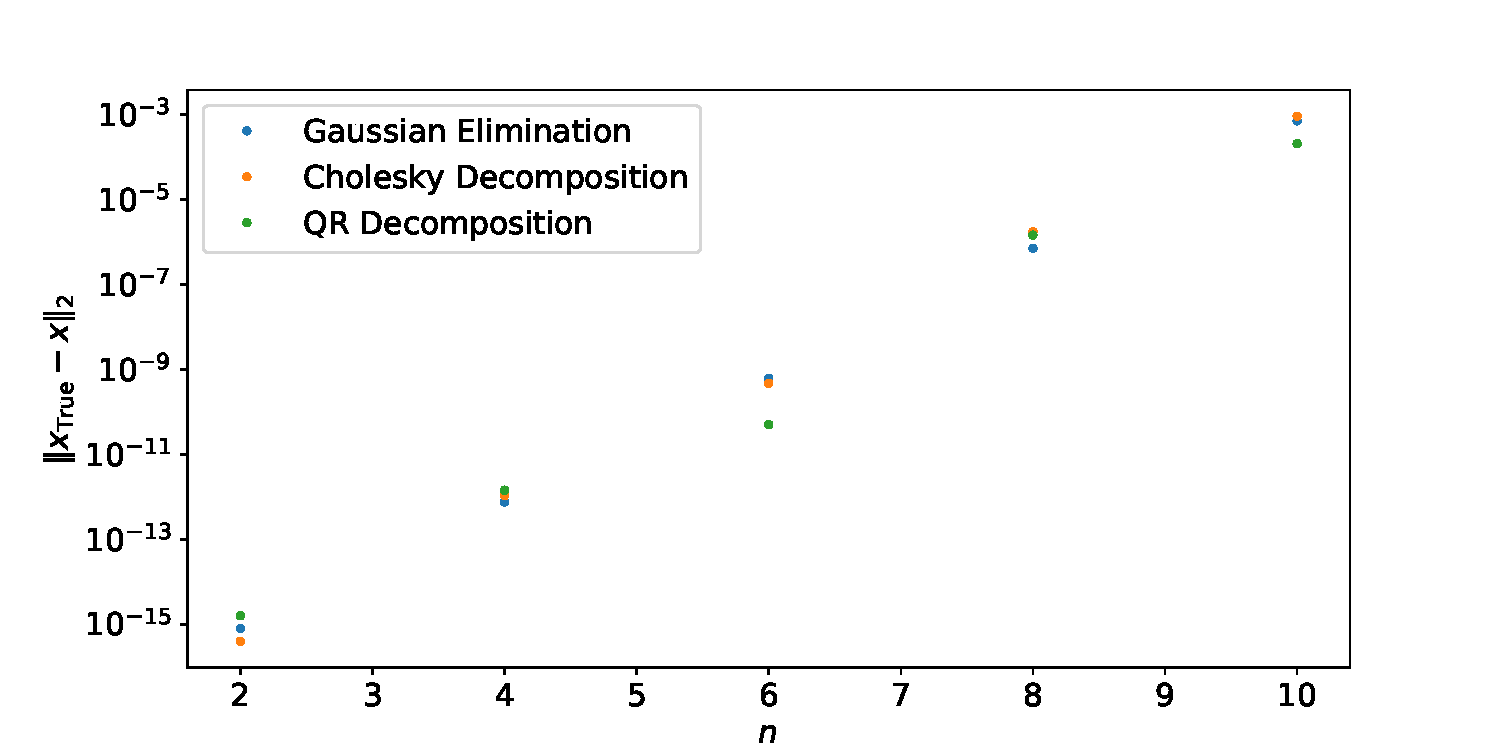
\includegraphics[width=\textwidth]{../5_6_7/7.pdf}
  \caption{Error of the numerical solutions for Hilbert matrices with
  growing $n$.}
  \label{fig:7}
\end{figure}

\end{document}
